\documentclass{article}
\usepackage{graphicx}
\graphicspath{{images/}}
\begin{document}

\title{mbeddr Header Importer Installation}
\author{Mohammadreza Basirati}
\maketitle

\section{Introduction}
Header Importer is a tool to import declarations from C header files into an mbeddr\footnote{More information about mbeddr on http://mbeddr.com/} project, so developers can use them in their code.
The need for such a tool came from this reason that mbeddr is based on JetBrains MPS\footnote{More information about MPS on https://www.jetbrains.com/mps/}. In MPS' editor, code text is a representation of the data node in the under laying xml and you cannot paste some text into the MPS' editor directly. So for using legacy codes, in this context a header file, we need a tool to import the codes into our mbeddr project.

Until now this tool has been tested only for the stdio.h file which comes with the importer and is located in the "headerimporter" folder.

\section{Installation}
\begin{itemize}
\item[Step 1]
The importer works as a tool for mbeddr, so as the first step you need mbeddr installed on your machine. For installing mbeddr see the link http://mbeddr.com/download.html or http://mbeddr.fortiss.org . JetBrains installation links and other prerequisites for mbeddr can be found there.
\item[Step 2]
Next step is to clone the importer project on your machine. Source code of the importer is on the github and can be accessed by this address: https://github.com/basirati/headerimporter.git. After cloning the repository you will find three folders, a readme.md file, and the stdio.h file. The folders are \texttt{scanner\_parser}, bparser, and STDIOImporter. The \texttt{scanner\_parser} folder contains the files for scanner and parser. In the bparser folder you will find a Java project that uses the scanner and parser and provides the results in a manner that the MPS importer project will be able to use Importer folder contains the MPS project of the importer. More details about these files and the structure of the importer will be discussed later.
\item[Step 3]
Next step is to open the STDIOImporter project from MPS. After opening the project you should first update the address of a jar file that the project uses it. Now the project has some errors (Figure 1). The jar file name is bparser.jar and it's located in bparser/out/artifacts/\texttt{bparser\_jar} folder. For updating the address proceed the following steps:

\begin{figure}[h]
\caption{Project With Errors}
\centering
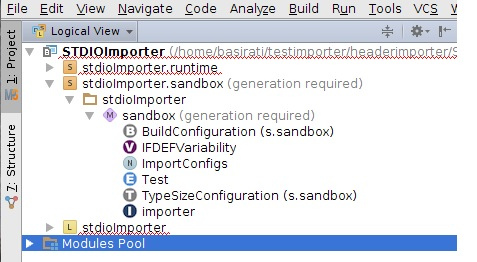
\includegraphics[scale=1]{errscreen.jpg}
\end{figure}

\begin{enumerate}
\item
Right-click on stdioImporter.runtime
\item
Go to Module Properties
\item
In the common tab you need to update the address of bparser.jar file, for doing this you need to follow these steps:
\begin{enumerate}
\item
In section Model Root there are two models. The first is default and the second is a \texttt{java\_classes} model. Bparser.jar file is located under this model (Right now it's red showing that it has some problems, Figure2)
\begin{figure}[ht]
\caption{Missing Jar State}
\centering
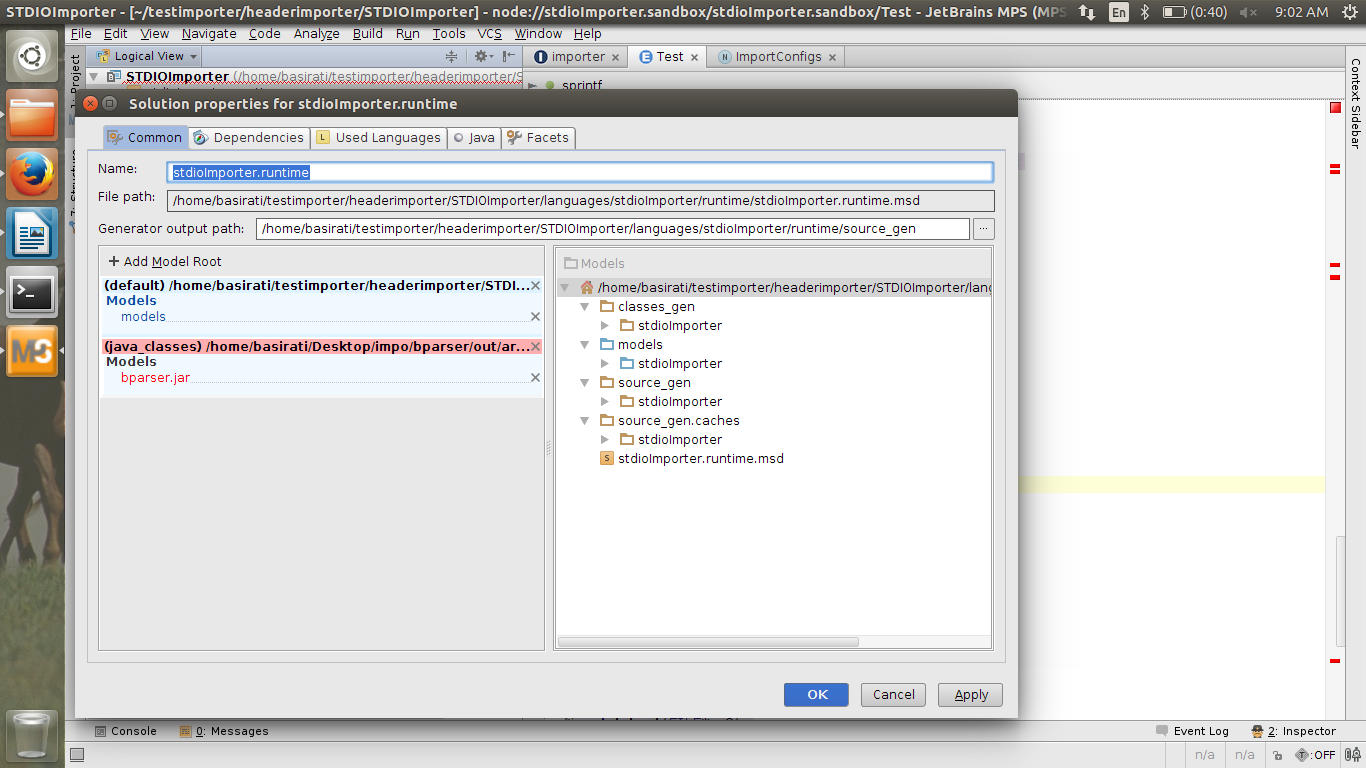
\includegraphics[scale=0.5]{jarmissed.jpg}
\end{figure}
\item
Click on the little cross on the bparser.jar line to delete the old version.
\item
Now click on the \texttt{java\_classes} model line. You will see the model browser window on the right is empty. Right click in the empty area.
\item
Right-click in the right small file browser on the right of the window.
\item
Click on "Change Root Folder".
\item
In the opened file browser select the folder containing the bparser.jar which is: ".../headerimporter/bparser/out/artifacts/\texttt{bparser\_jar}" (Figure 3).
\begin{figure}[h]
\caption{bparser.jar Path Selection}
\centering
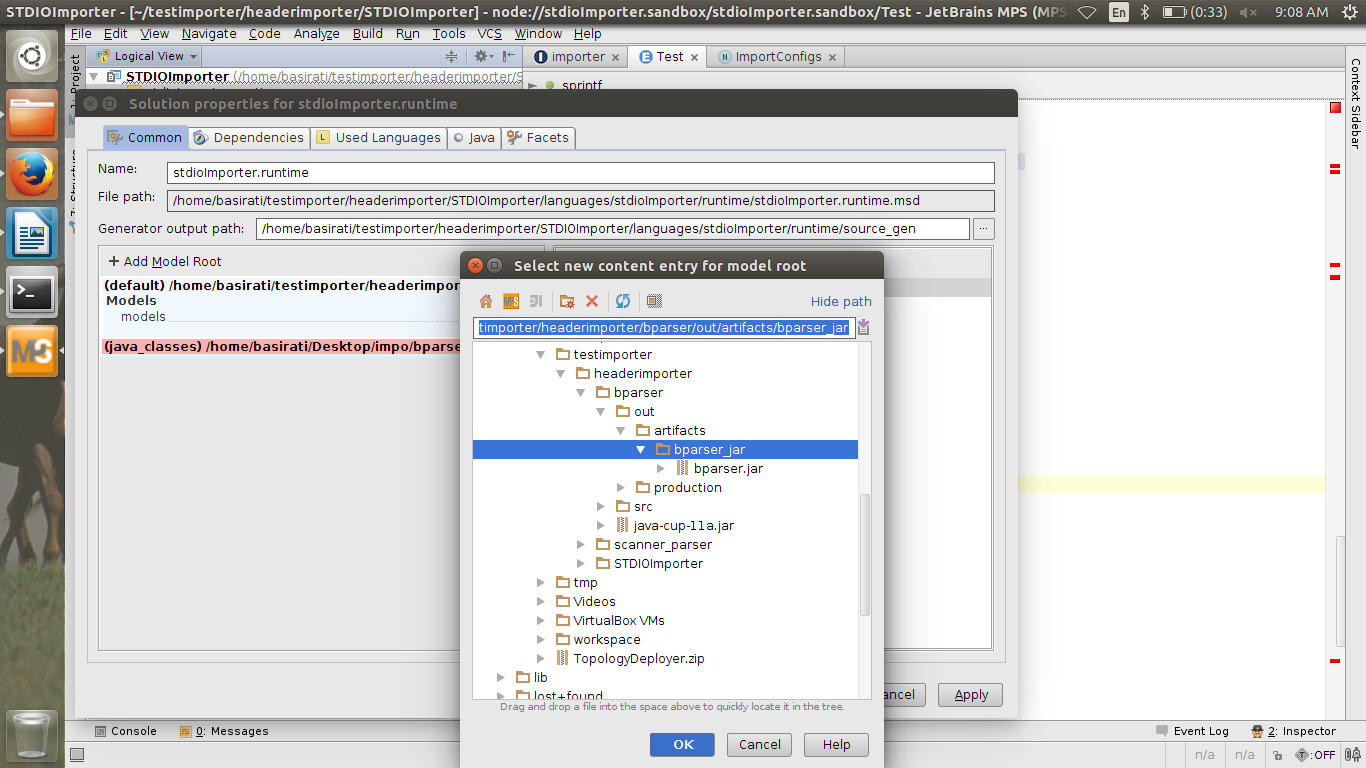
\includegraphics[scale=0.3]{selectpath.jpg}
\end{figure}
\begin{figure}[h]
\caption{Updated Jar State}
\centering
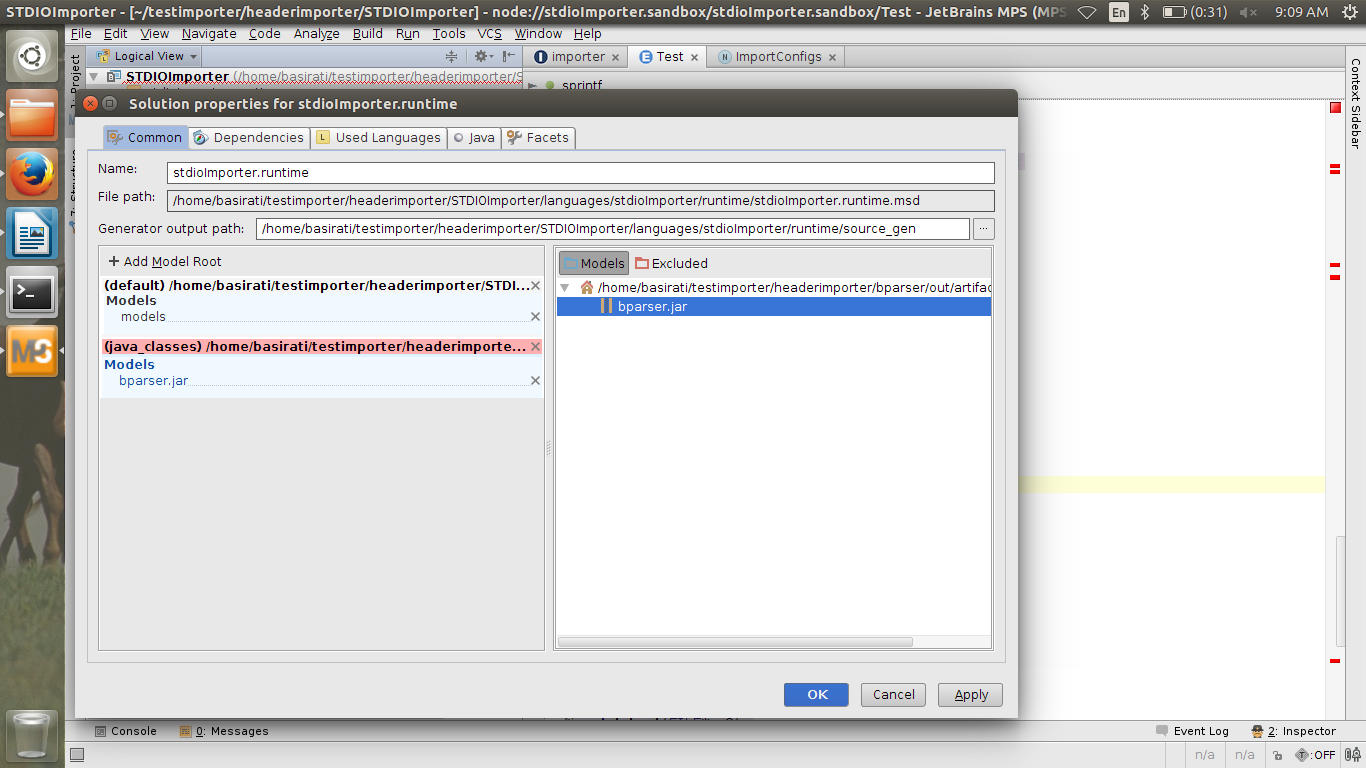
\includegraphics[scale=0.4]{correctjar.jpg}
\end{figure}
\item
Now in the small file browser you should be able to see the bparser.jar file.Right-click on the bparser.jar file and select Models.
\end{enumerate}
\item
Now go to the tab Java. In the libraries section also you need to update the address of bparser.jar. Remove the old bparser.jar by selecting it and clicking on the minus sign on the right of the window (Figure 5).
\begin{figure}[h]
\caption{Java Library Missed Jar State}
\centering
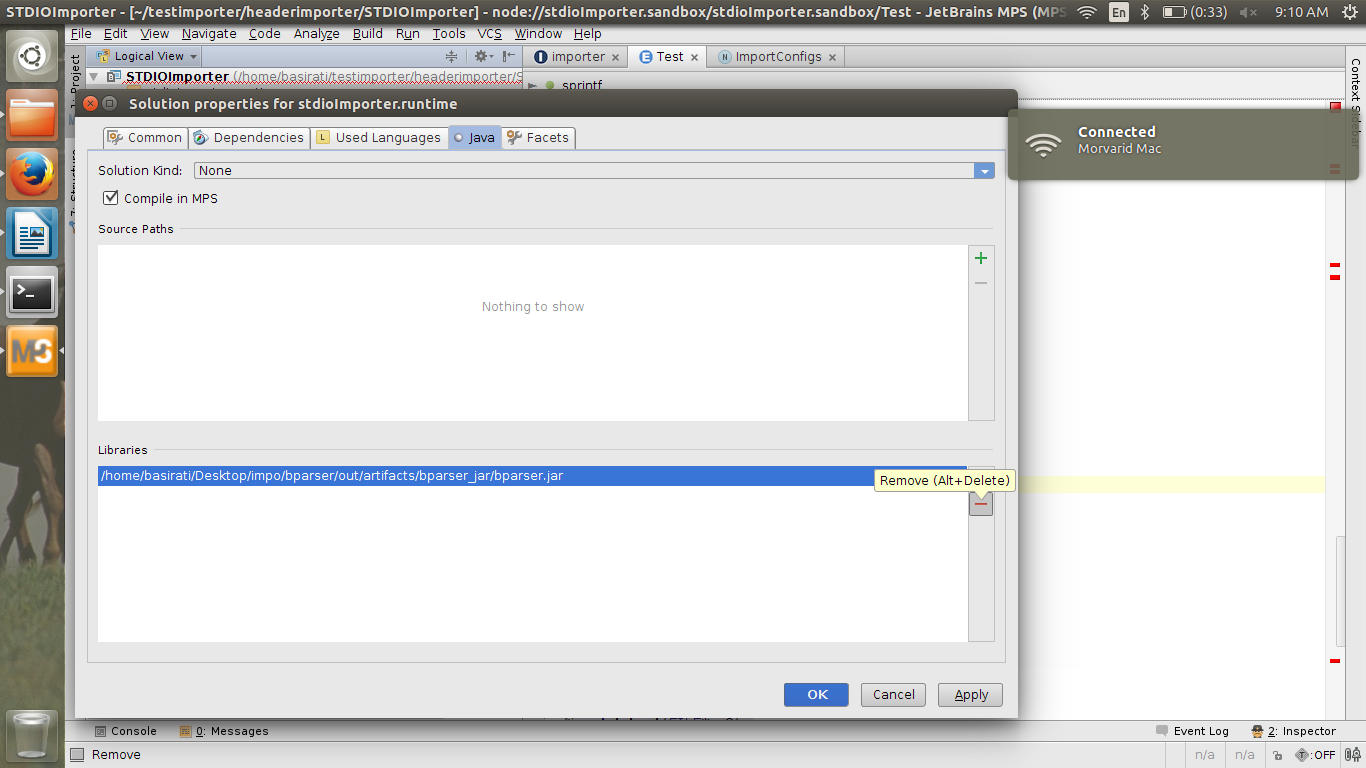
\includegraphics[scale=0.4]{javalibmissed.jpg}
\end{figure}
\item
Now add the new bparser.jar file by clicking on the plus sign and selecting the file in this address:”.../importer-stdio/bparser/out/artifacts/\texttt{bparser\_jar}/bparser.jar”
\item
A dialog will be displayed (Figure 6). Click the OK button.
\begin{figure}[h]
\caption{Opened Dialogue Window}
\centering
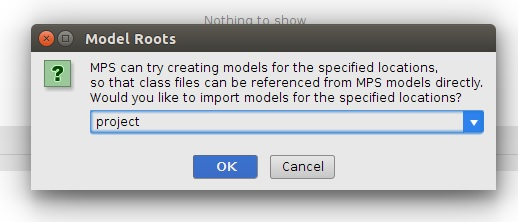
\includegraphics[scale=0.5]{dialog.jpg}
\end{figure}
\item
Now click on apply and the ok buttons.
\item
Now your project should not have any errors.  As the next step you need to rebuild the whole project by right-clicking on the STDIOImporter node and then clicking the rebuild STDIOImporter.
\item
Now the importer is ready to use.
\end{enumerate}
\end{itemize}


\end{document}
